\chapter{Introducción}
\label{chap:introduccion}

La enfermedad de Parkinson es un trastorno neurodegenerativo que afecta a millones de personas en todo el mundo, con una incidencia especialmente alta en personas de edad avanzada \cite{fuente_parkinson_epidemiologia}. Para estos pacientes, la rehabilitación física es clave para mantener su calidad de vida, pero el acceso a estas terapias a menudo supone un desafío considerable. Esta problemática se agrava en zonas rurales o despobladas, donde la distancia a los centros de salud y la dependencia de terceros para el desplazamiento complican o incluso impiden la continuidad del tratamiento, afectando negativamente a la evolución del paciente.

En este contexto, la telerehabilitación surge como una solución cada vez más necesaria para superar las dificultades de desplazamiento y la saturación de los servicios sanitarios \cite{cottrell2017telerehabilitation}. Este Trabajo de Fin de Grado se enmarca en el proyecto de investigación \textbf{FIS PI19/00670} \cite {garrido_fisfbis}, en colaboración con el Hospital Universitario de Burgos (HUBU), que busca precisamente mejorar las terapias a distancia para estos pacientes.

El punto de partida de este trabajo es un sistema previo, desarrollado en el marco del proyecto mencionado, que ya permitía un análisis básico de los ejercicios grabados en vídeo. Sin embargo, su infraestructura tecnológica presentaba limitaciones de escalabilidad y fiabilidad que dificultaban su uso a gran escala. El objetivo principal de este TFG es, por tanto, el rediseño y la construcción de un \textit{backend} mucho más robusto, capaz de procesar múltiples flujos de vídeo de forma eficiente y estable, sentando así las bases para un futuro sistema de \textit{feedback} automático fiable.

Para conseguirlo, se ha diseñado e implementado una nueva arquitectura basada en los paradigmas de microservicios y procesamiento de datos a gran escala. La solución implementa un \textit{pipeline} de datos que orquesta la captura de las sesiones de vídeo, su transporte a través de un sistema de mensajería distribuida y su posterior análisis mediante un motor de computación en clúster. Toda esta infraestructura se ha empaquetado mediante tecnologías de contenerización para garantizar un despliegue consistente, reproducible y fácilmente escalable.

\begin{figure}[H]
    \centering
    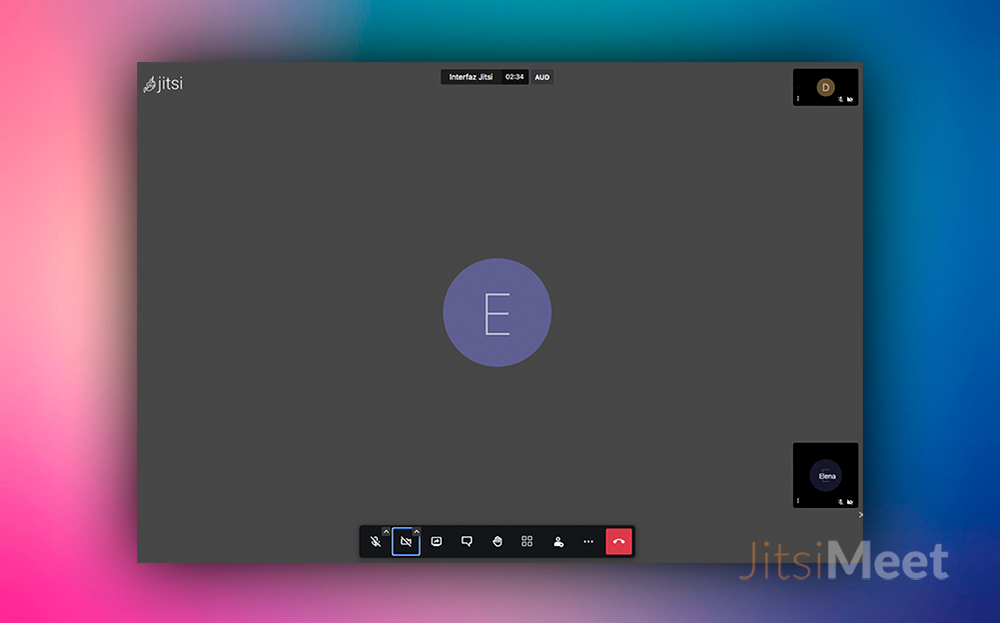
\includegraphics[width=0.8\textwidth]{img/interfazjitsi.jpg}
    \caption{Ejemplo de la interfaz de Jitsi Meet, la plataforma de videoconferencia utilizada para las sesiones de tele-rehabilitación.}
    \label{fig:interfaz_jitsi}
\end{figure}

La presente memoria documenta todo el proceso de investigación, diseño y desarrollo llevado a cabo. El Capítulo \ref{chap:objetivos} detalla los objetivos generales y técnicos del proyecto. En el Capítulo \ref{chap:conceptos} se exponen los fundamentos teóricos de las tecnologías empleadas. El Capítulo \ref{chap:herramientas} describe en profundidad las herramientas y la metodología de trabajo utilizadas. El Capítulo \ref{chap:desarrollo} narra los aspectos más relevantes del desarrollo, incluyendo los desafíos encontrados y las decisiones de diseño tomadas. Finalmente, el Capítulo \ref{chap:conclusiones} presenta las conclusiones extraídas del trabajo realizado y propone posibles líneas de trabajo futuras.